\section{Result III: Context Is Not the Explanation}
\label{sec:representation}

The behavioural results above admit an alternative reading in which
UWM-JEPA owes its separation to a stronger context encoder rather than
to its predictor. The held-out probe in this section tests that
reading directly. UWM-JEPA and a parameter-matched LSTM-JEPA agree
within seed noise on the same probe, which locates the empirical
separation in the predictor rather than in encoder quality.

\subsection{Held-out context probe}

We freeze each trained encoder, take the latent produced on a short
context window, and fit a linear probe to predict the hidden velocity
of the next step~\cite{alain2017understanding}. Training and evaluation
splits are disjoint across trajectories and the probe is linear, so the
metric reflects information in the encoder's representation rather than
downstream nonlinear capacity. Figure~\ref{fig:heldout} reports
five-seed results.

\begin{figure}[t]
  \centering
  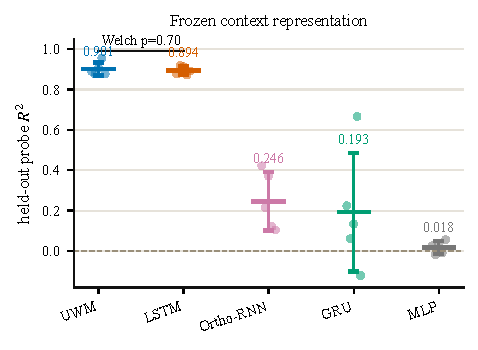
\includegraphics[width=\linewidth]{figures/fig_heldout_probe.pdf}
  \caption{\textbf{Held-out linear-probe $R^2$ on hidden velocity
  (five seeds).} UWM-JEPA ($0.901 \pm 0.032$) and LSTM-JEPA
  ($0.894 \pm 0.021$) are not significantly different
  (Welch $p=0.70$). The density-matrix latent is not a win on context
  probing alone; the orthogonal, GRU, and MLP baselines fall far below.}
  \label{fig:heldout}
\end{figure}

The two top entries in \cref{fig:heldout} sit within error of each
other: UWM-JEPA at $0.901 \pm 0.032$, LSTM-JEPA at $0.894 \pm 0.021$,
with Welch $p=0.70$. A well-regularised recurrent encoder already
recovers nearly all of the probe-accessible information about
hidden velocity in this domain, so the density-matrix latent confers
no context-probing advantage. The three non-recurrent baselines in
the same figure (orthogonal~\cite{arjovsky2016unitary,wisdom2016full},
GRU~\cite{cho2014learning}, and MLP at $0.246 \pm 0.144$,
$0.193 \pm 0.293$, and $0.018 \pm 0.032$) confirm that the probe
discriminates: it places the two strong recurrent and density-matrix
encoders together at the top and the weaker baselines well below them.
The GRU variance is large, so its mean is not interpreted sharply; the
relevant point is that the UWM--LSTM tie at the top reflects shared
high probe quality, not a ceiling on the probe itself.

\paragraph{Consequence}
Since the context probe ties, the remaining experiments evaluate the
predictor rather than the encoder. We test whether predicted future
latents retrieve the right target latent, whether frozen probes retain
hidden-state information after blind rollout, and whether counterfactual
actions move the latent in the expected direction. Collapse diagnostics
and anti-collapse sweeps are reported in the supplement; they confirm
that the UWM-JEPA runs used here remain non-collapsed under the tested
regularisation protocols but use different regulariser variants and
checkpoint protocols, so they are not directly comparable to the
five-seed context-probe numbers in \cref{fig:heldout}.
